
\begin{figure}[ht]
    \centering
    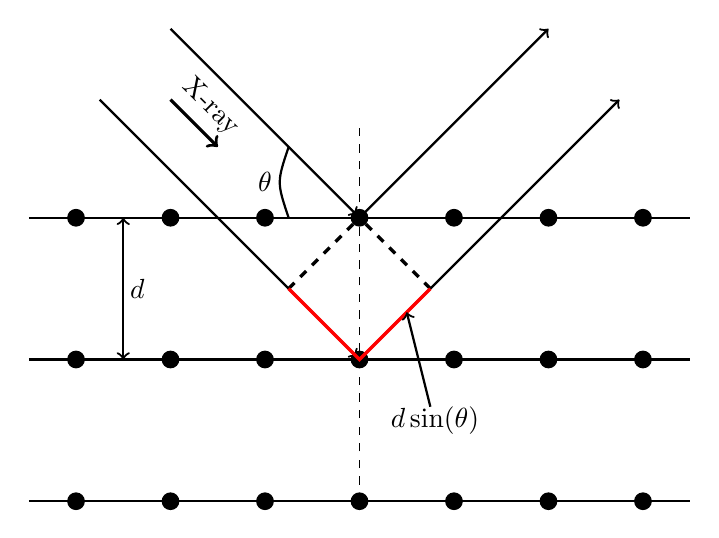
\begin{tikzpicture}[scale=0.6]
        \draw[thick] (-7,-3) -- (7,-3);
        \draw[thick] (-7,0) -- (7,0);
        \draw[thick] (-7,3) -- (7,3);
        
        %\draw (-15,-15) grid (15,15);
        \foreach \y in {-3,0,3}
            \foreach \a in {-6, -4, -2, 0, 2, 4, 6}
                \filldraw [black] (\a,\y) circle (5pt); 
        
        \draw[thick, ->] (-4, 7) -- (-0.05,3.05);
        \draw[thick, ->] (0,3) -- (4, 7);
        \draw[thick, ->] (-5.5, 5.5) -- (-0.05,0.05);
        \draw[thick, ->] (0,0) -- (5.5, 5.5); 
        
        \draw[very thick, dashed] (-1.5,1.5) -- (0,3);
        \draw[very thick, dashed] (1.5,1.5) -- (0,3);
        
        %Angle
        \draw[thick] (-1.5,4.5) .. controls (-1.75, 3.75) .. (-1.5, 3);
        \node at (-2, 3.75) {$\theta$};
        %\node at (0,3.5) {0,3};
        \draw[dashed] (0,-3) -- (0,5);
        \draw[thick,->] (-5,3) -- (-5,0);
        \draw[thick,->] (-5,0) -- (-5,3);
        \node at (-4.7, 1.5) {$d$};
        
        \draw[very thick, red] (-1.5,1.5) -- (0,0) -- (1.5,1.5); 
        \draw[thick, ->] (1.5,-1) -- (1,1);
        \node at (1.6,-1.3) {$d\sin(\theta)$};
        
        \draw[very thick, ->] (-4,5.5) -- (-3,4.5) node[midway, left, above, rotate=-45]{X-ray};
    \end{tikzpicture}
    \caption{Caption}
    \label{fig:test}
\end{figure}


\subsubsection{Electrical conduction}

It is common practice to divide materials into categories regarding their electrical properties such as insulators, semiconductors and conductors. The differences in these properties originate from the band structures described by quantum mechanics **FIGURE**

*An insulator has a completely filled valence band and an empty conduction band with a large band gap, while conductors have a  partially filled valence band (metal) or overlapped bands (semi-metal), thus helping electrons in the crystal move more easily when an external field is applied.*
